\documentclass[10pt]{article}

\usepackage{spheric}
%%%TITLE
\title{A dynamic refinement strategy in SPH for simulating the water entry of an elastomer}
\date{}

%%AFFILIATIONS
\author[$\relax$]{Lu Wang}
\author[$\relax$]{Fei Xu$^\dagger$}
\author[$\relax$]{Yang Yang}

\affil[$\relax$]{School of Aeronautics, Northwestern Polytechnical University, 710072, Xi'an, P. R. China}

\affil[$\relax$]{\email{\dagger}{xufei@nwpu.edu.cn}}


%%DOCUMENT
\begin{document}

\maketitle

%\SelectedTopics{}

%%PLEASE PUT YOUR ABSTRACT HERE
\begin{abstract}
As a fully Lagrangian particle method, SPH's major advantage for the FSI (Fluid-Structure Interaction) issue is that the highly nonlinear behavior of the motion of the interface can be implicitly captured with a sharp interface. Naturally, extensive computation is needed due to the massive particles used to capture the interface precisely. In the Eulerian and Lagrangian mesh methods, the variable resolution that preserves high computational efficiency and accuracy has been implemented in both structured and unstructured meshes. Similarly, achieving variable resolution has been an important step in the development of the SPH method. It can not only describe the physical field more minutely but also decrease the computational cost because of the finer spatial resolution and the local refinement. To decrease the cost and to capture the interface between the fluid and structure, this paper provides a general dynamic refinement strategy including refinement pattern and relevant parameters as shown in Fig. \ref{fig:29}, and a new refinement criterion aiming at the FSI problems is proposed to catch the interface more exactly.

When we simulate a FSI problem by SPH method, the structure is generally treated as a rigid body rather than an elastomer. There is not much research on interaction between elastomers and fluid in SPH. Therefore, we apply the previous proposed dynamic refinement strategy to the water entry of an elastic beam. By measuring the energy, acceleration and surface pressure of the elastic beam, the results indicate that this new strategy can obtain remarkable accuracy and efficiency. In addition, in order to deal with the interface accurately, we apply an improved FPM method (the developed method of SPH) to the vicinity of the interface, which shows remarkable results.

\begin{figure}[!htb]
\centering
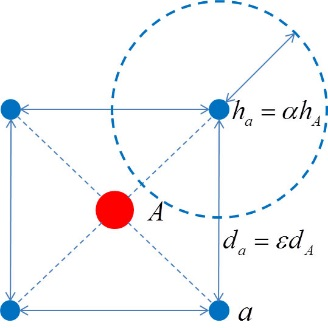
\includegraphics[width=0.4\textwidth]{29-1.png}
\caption{Splitting pattern in dynamic refinement strategy}\label{fig:29}
\end{figure}

\end{abstract}


%%THE END OF ABSTRACT

\addbib

\end{document}
